% lithium ion: lithium cobalt oxide / graphite
\chapter{Procedure}
The experimental procedures aimed to progressively change the cell's state of charge and state of health systematically, such that the influence of each on shift in acoustic ToF through the cell would be observable.
The goal of the first experiment was to acoustically observe first shifts in ToF data due to change in a cell's state of charge, and then shifts due to cycling-induced lithium plating, a form of change of the cell's state of health. 
It was unsuccessful due to overwhelming noise from uncontrolled ambient conditions. 
In response, several improvements were made to the experimental apparatus in an attempt to eliminate appreciable noise in the ToF data due to ambient conditions. 
The second experiment's goal was to determine whether these changes adequately controlled the ambient conditions to prevent them from overwhelming the ToF data with noise; it was successful. 
The experiment showed a close and consistent relationship between time of flight and cell state of charge (ToF and SoC).

Recall that three three main actors of change on an acoustic wave's time of flight through a battery cell are ambient conditions (temperature and pressure), state of charge, and state of health, as shown by the prior literature such as \cite{SOC-SOH-EST}, and the fact that acoustic velocity through a material is constant at a given temperature and pressure \cite{OLYMPUS}. Now that the set-up was validated to have minimal change in ambient conditions, and a relationship between ToF and SoC strongly established, further experimentation could reasonably explore the relationship between the cell's state of health and acoustic time of flight. The goal of the next experiment was to force plating via aggressive electrochemical cycling, and acoustically observe this while it happens using ToF data; it was successful. Following that, the goal of the next fourth experiment was to induce a minimum of plating on the cell, to use as a point of comparison; this was accomplished by cycling the cell at 5C but never 10C rates of charge. The subsequent goal was to induce just some plating in the cell, by loading at a 10C charge rate for only one charging cycle; it was successful. Then, to build up more data for analysis, potentially for use in controlling for the influence of temperature, a cell was cycled at C/2.5 20 times, before being destructively cycled at progressively higher rates until 10C.

\section{Observing ToF Shifts Due to State of Charge}

\subsection{Acoustic Monitoring of Cell Cycling in Unsteady Conditions}

The cell was cycled (charged and discharged) five times at a C/2.5 rate. 
Both the battery cell and the transducers used to send and receive the acoustic waves are subject to changes in operating characteristics due to change in temperature, so each testing protocol begins with a long rest to give the unit under test and the testing equipment time to acclimate to the ambient conditions. 
Then, the cell charges at a constant-current rate of 0.0120 Amps. 
The C/2.5 rate was chosen because such a gentle rate would induce no appreciable lithium plating, so the state of health of the cell would be roughly constant. 
If the cell's state of health did not change between cycles, and the experiment's ambient conditions held steady, then all changes in acoustic time of flight can be assumed to be due to change in state of charge.
The cycle then rested ten minutes, was discharged using the same constant-current C/2.5 protocol, and then rested for ten minutes again. 
The rests between and within cycles allow for the cell to reach new steady-state conditions. 
There was a potential for the cell to experience somewhat significant transient effects due to phenomena such as the heat addition or structural stiffening experienced during the oxidation-reduction reaction of cyclic charging and discharging; the rest cycles give the cell time to relax and modulate.
The full rest-charge-rest-discharge sequence was repeated for a total of five cycles.

Unfortunately, the assumption that the ambient conditions were steady did not hold, leading to considerable noise in the in the readings due to environmental interference. The noise ultimately drowned the acoustic ToF signal.

\subsection{Acoustic Monitoring of Cell at Rest in Unsteady Conditions}\label{chamberTest}
Since it was impossible to determine the source of changes in ToF data for the prior test, or to determine what was signal and what was noise, a more piecewise approach to building up the experiment was needed. Due to the very small size of the cell, small variations in temperature and pressure could theoretically have relatively large impacts on the speed with which high-frequency acoustic waves travel through the cell. Some possible solutions were: passively or actively controlling the temperature to be much more constant, better regulating the pressure applied to the cell, and using higher frequency transducers to probe the cell. Switching the 2.5MHz transducers for 15MHz transducers was quick and easy since the second set of transducers was already on hand, so this was done for the next experiment. Additionally, the relatively loosely fluctuating ambient temperature was expected to have a relatively large effect on time of flight, so the pressurizing apparatus was inserted into a thermal chamber, as described in \hyperref[thermalChamber]{\cref{thermalChamber}}. The stack pressure variation is expected to a small fraction of an MPa and expensive to improve, so this was left unchanged, to be revisited only if necessary.

Additionally, the cycling was postponed to a later experiment.
For now, the cell would be left at rest for the duration of the experiment. 
If there was no significant shift in acoustic ToF data while the cell waited at rest for a long period, then the noise in the environment is adequately controlled and cycling experimentation can proceed. 
If there were still shifts, the environment would need further control, probably through higher-precision active temperature control and pressure control. 
For 24 hours, the cell was probed ultrasonically while pressurized in the thermal chamber.

The data show that the ToF did not shift while the temperature was held constant, and then shifted in step with a shift in temperature at the end, verifying that this setup effectively reduced environmental noise to acceptable levels to begin attempting to observe ToF shifts due to cell state.

\subsection{Experiment A: Acoustic Monitoring of Electrochemical Cycling}
\begin{figure}[h!]\label{fig:neware0309}
    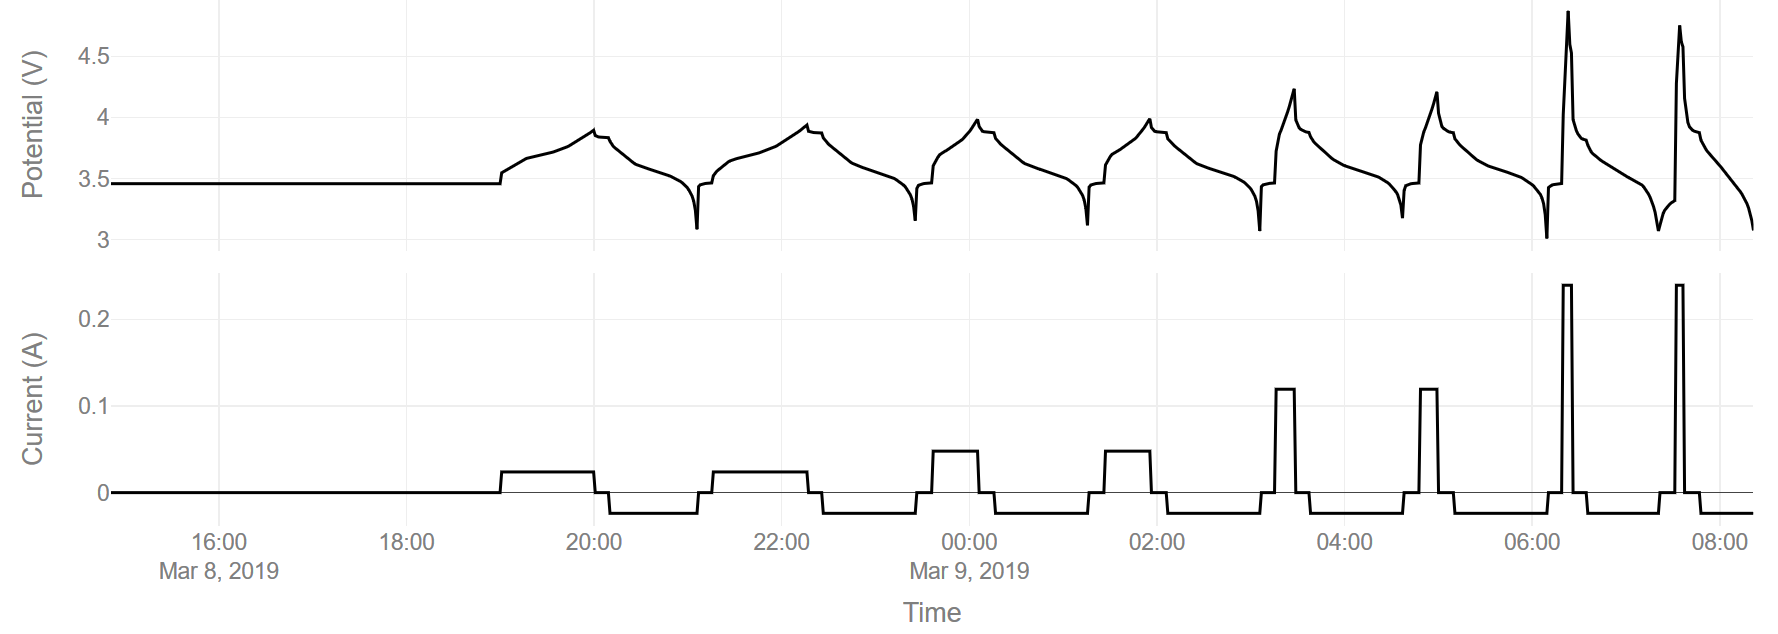
\includegraphics[width=0.75\textwidth]{Thesis/neware0309.PNG}
    \centering
    \caption{The protocol for experiment A.}
\end{figure}
Once the noise levels were brought under control, attempting to observe change of state via acoustic ToF shift could begin. The cycle was set up as in the first experiment, with a long initial rest period to ensure starting conditions were steady state, then five cycles consisting of a 10 minute rest, a C/2.5 current-controlled charge, another 10 minute rest, and then a C/2.5 current-controlled discharge. 
The system was kept pressurized to 2.4 PSI, which was a stack pressure of about 0.42MPa, falling into Cannarella's low stack pressure regime.

Once confirmed that the experimental set-up was capable of observing change of state of charge of the cell, it could also be investigated whether it could observe changes in state of health.

This intentionally reckless operation would force significant lithium plating to develop on the anode. 
After a rest to ensure steady-state conditions, the cell was given a ten minutes rest, charged at a 1C rate for 60 minutes, given 10 minutes rest, and discharged at a C/2 rate. 
This sequence was repeated once, for two total cycles. 
It was then repeated with a charging protocol of 2C for 30 minutes, then 5C for 12 minutes, then 10C for 6 minutes. 
The latter two cycles expect lithium plating.

\section{Observing ToF Shifts Due to State of Health} 
\subsection{Experiment B: Acoustic Monitoring of Lithium Plating}
\begin{figure}[h!]\label{fig:neware0325}
    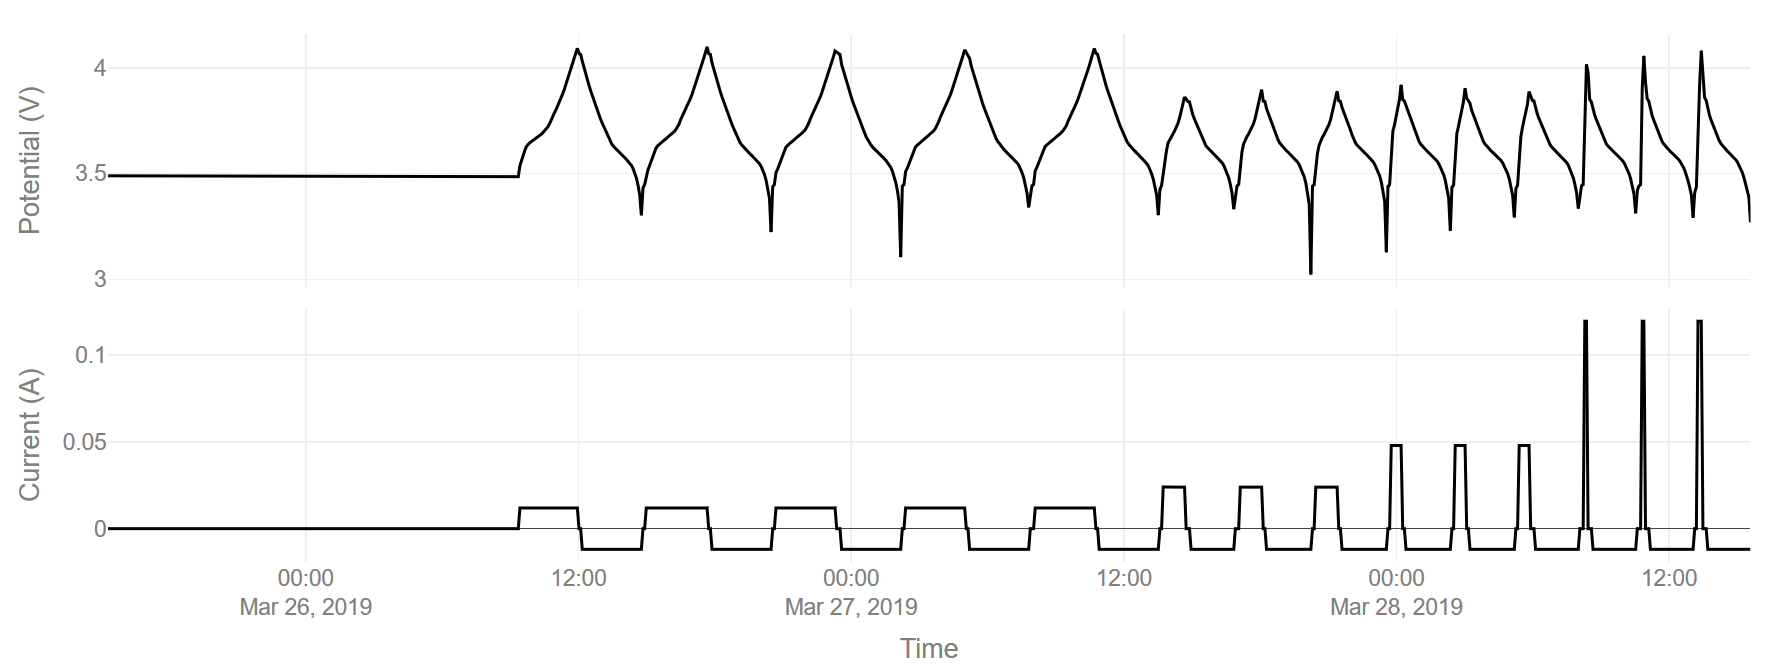
\includegraphics[width=0.75\textwidth]{Thesis/neware0325.PNG}
    \centering
    \caption{The protocol for experiment B.}
\end{figure}

The goal of this test was to plate lithium at less aggressive charging rates of 5C, rather than 10C, so that most or all appreciable plating would be removed during the discharge cycle. XPS and SEM analysis showed this to be mostly successful. However, the temperature fluctuated much more during this experiment than the prior, and this lead to noisy readings of time of flight. This created an opportunity to relate change in ambient temperature with change in time acoustic time of flight. 

\subsection{Experiment C: Acoustic Monitoring of Minimal Lithium Plating}
\begin{figure}[h!]\label{fig:neware0409}
    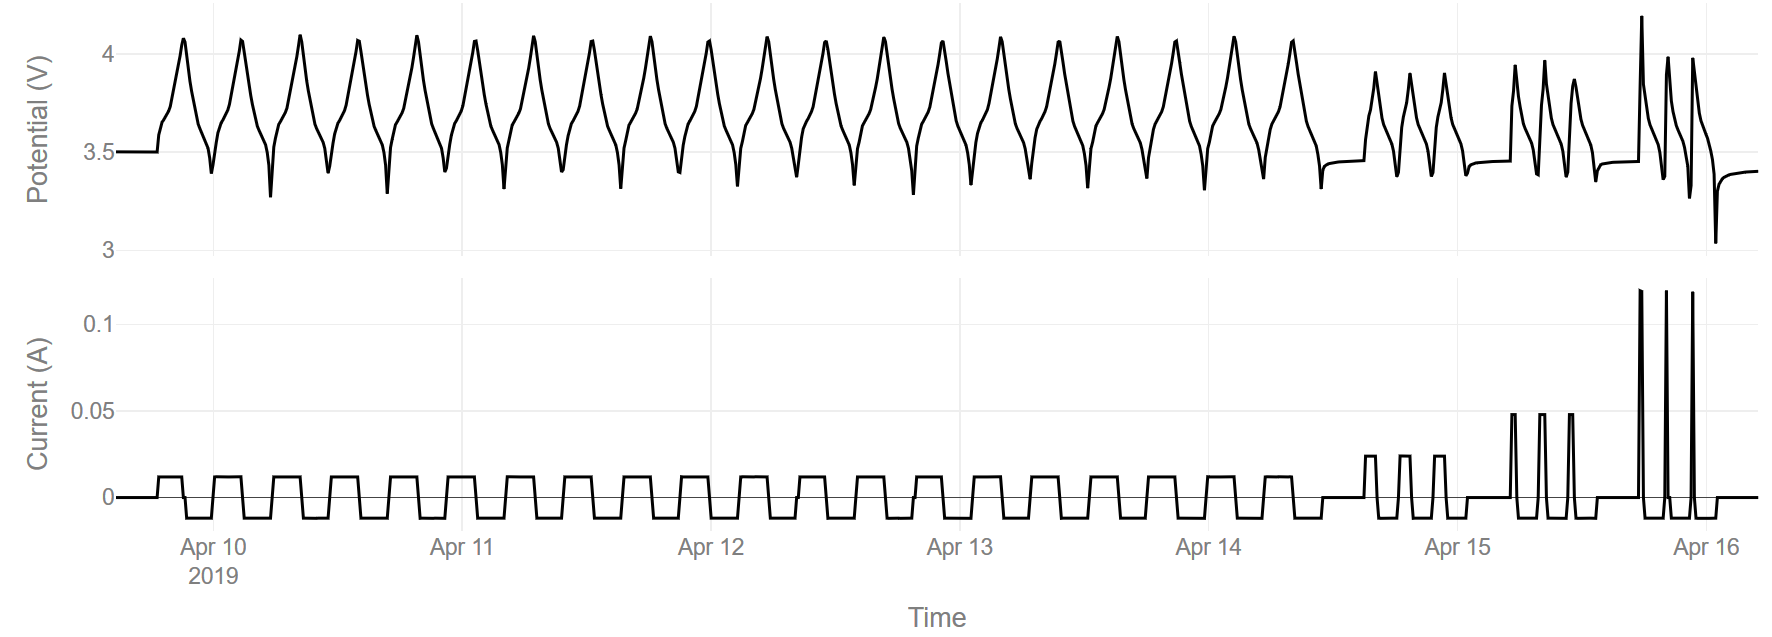
\includegraphics[width=0.75\textwidth]{Thesis/neware0409.PNG}
    \centering
    \caption{The protocol for experiment C.}
\end{figure}
The goal of this experiment was to plate a fixed amount of lithium. It used a protocol similar to the earlier plating protocol, but with only one cycle of charging at the 10C rate. One hiccup during this experiment was that the thermocouples stopped logging data for much of the experiment. 


\subsection{Experiment D: Acoustic Monitoring of Gentle Cycling}
\begin{figure}[h!]\label{fig:neware0417}
    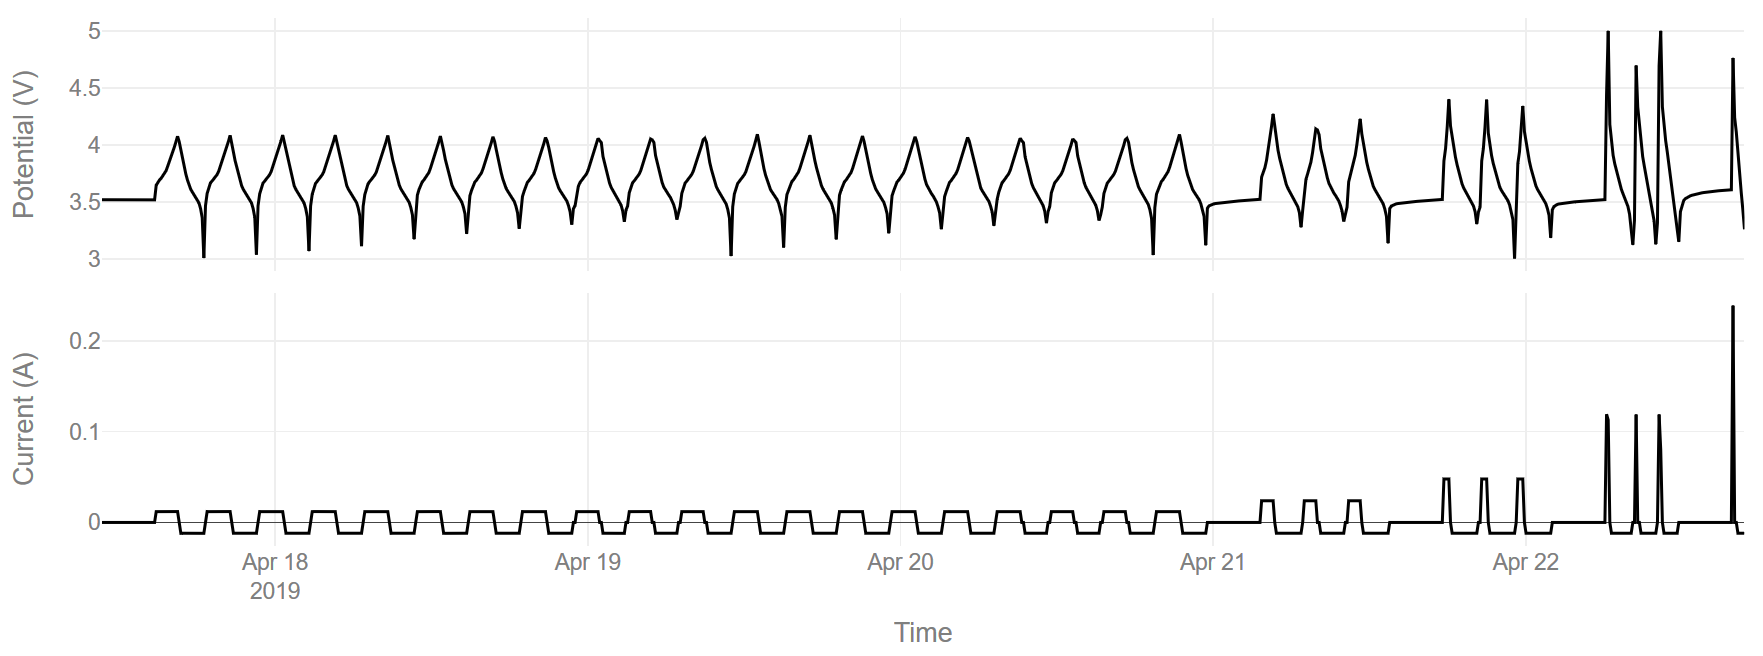
\includegraphics[width=0.75\textwidth]{Thesis/neware0417.PNG}
    \centering
    \caption{The protocol for experiment D.}
\end{figure}
This experiment aimed to increase the bank of data available for analysis. Previous experiments suggested that there could be a quantifiable relationship between change in ambient temperature and change in ToF shift, but there was too little data available free from the interference of cell state of health changes. This experiment ran 20 C/2.5 cycles before moving on to plating cycles. While not all the data was usable due to temperature logging issues, enough of the cycles had sufficient data.